% CSE 493S/599S Homework 1 — deliverables (Parts 0--1.4)
% Compile from repository root: pdflatex deliverables.tex

\documentclass[11pt]{article}
\usepackage[margin=1in]{geometry}
\usepackage{graphicx}
\usepackage{booktabs}
\usepackage{url}
\usepackage{hyperref}

\title{CSE 493S/599S HW1 --- Deliverables (Parts 0--1.4)}
\author{}
\date{}

\begin{document}
\maketitle

\section*{Part 0: Training infrastructure and sanity checks}

\subsection*{Code and artifacts}

\begin{itemize}
  \item \textbf{Training/inference:} \texttt{train.py}, \texttt{inference.py}, \texttt{model.py} (\texttt{key\_padding\_mask}), \texttt{tokenizer\_utils.py}, \texttt{part\_0\_1\_contract.py}.
  \item \textbf{Configs:} \texttt{configs/sanity\_quick.yaml}, \texttt{configs/sanity\_suffix\_quick.yaml} (and non-quick variants). Each run writes \texttt{config\_resolved.yaml}, \texttt{metrics.csv}, \texttt{tokenizer.json}, and \texttt{ckpt\_<step>.pt}.
\end{itemize}

\subsection*{Commands executed (verification)}

\begin{verbatim}
python train.py --config configs/sanity_quick.yaml
python train.py --config configs/sanity_suffix_quick.yaml
python inference.py --checkpoint_dir runs/sanity_quick_test --prompt "" --max_new_tokens 64
python inference.py --checkpoint_dir runs/sanity_suffix_quick --prompt "I l" --max_new_tokens 64
\end{verbatim}

\noindent
\textbf{Observed outputs:} greedy decode from BOS-only reproduced \texttt{I love machine learning}; decode with prefix \texttt{I l} reproduced the full line. Final logged metrics for memorization show train loss $\approx 6\times 10^{-5}$ and token/equation accuracy~1 on train/val/test (\texttt{runs/sanity\_quick\_test/metrics.csv}).

\subsection*{Figures}

\begin{figure}[h]
  \centering
  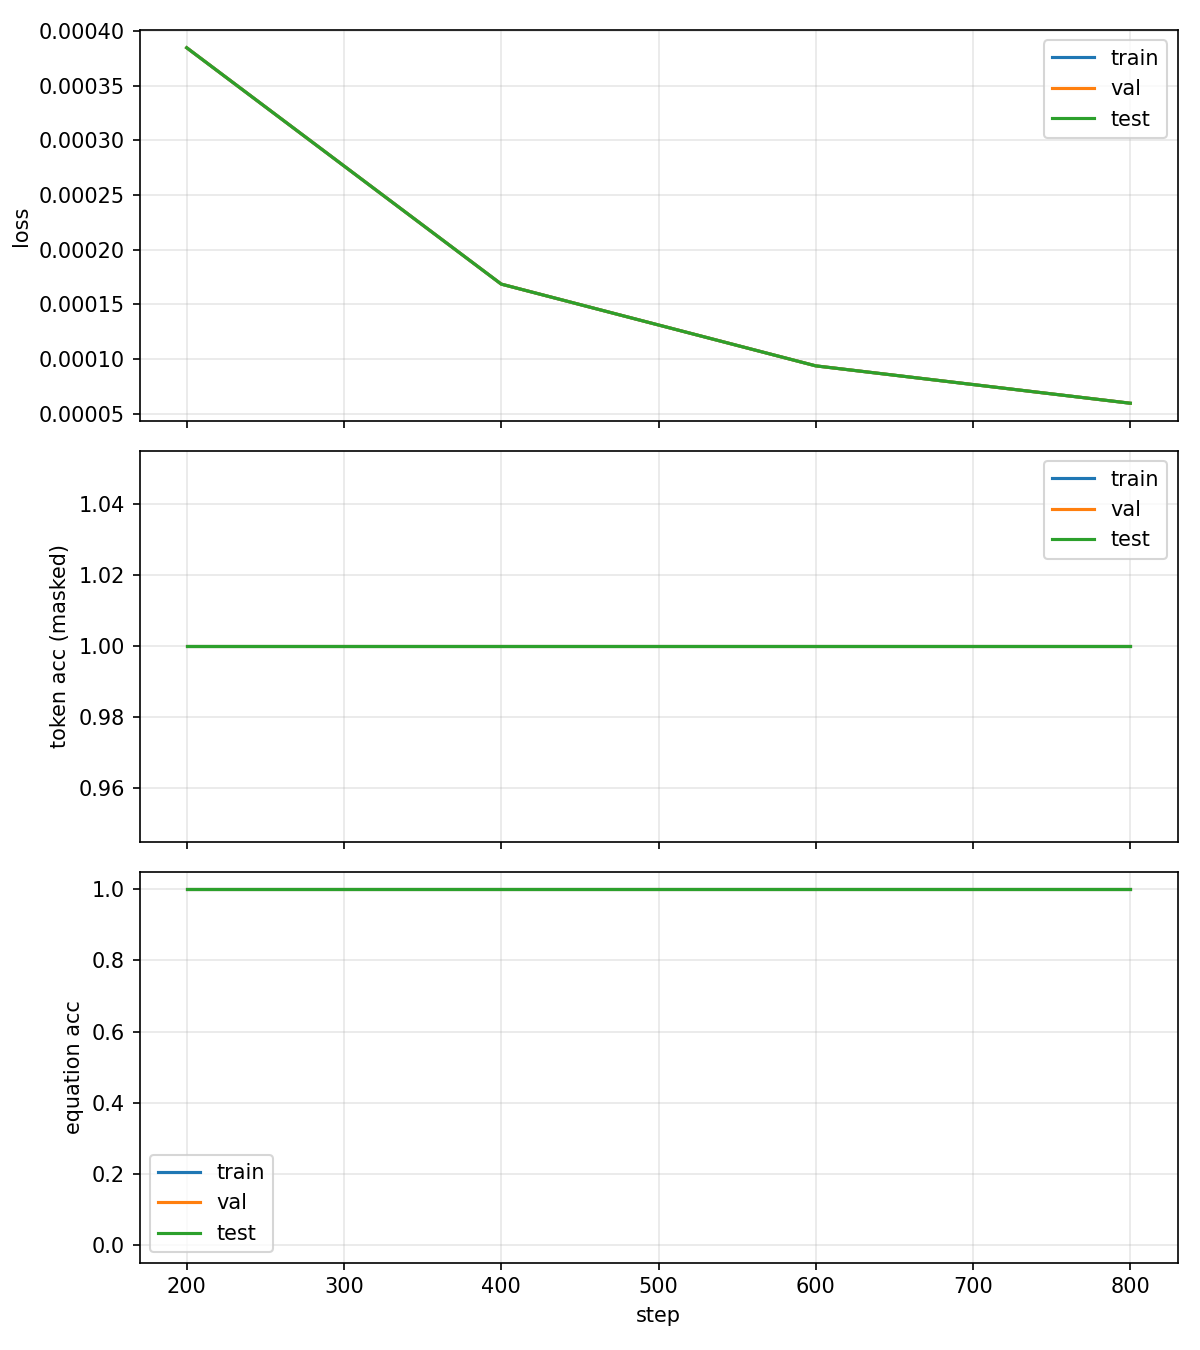
\includegraphics[width=0.85\linewidth]{figures/sanity_memorize.png}
  \caption{Sanity memorize run: loss and accuracy vs.\ step (\texttt{runs/sanity\_quick\_test}).}
\end{figure}

\begin{figure}[h]
  \centering
  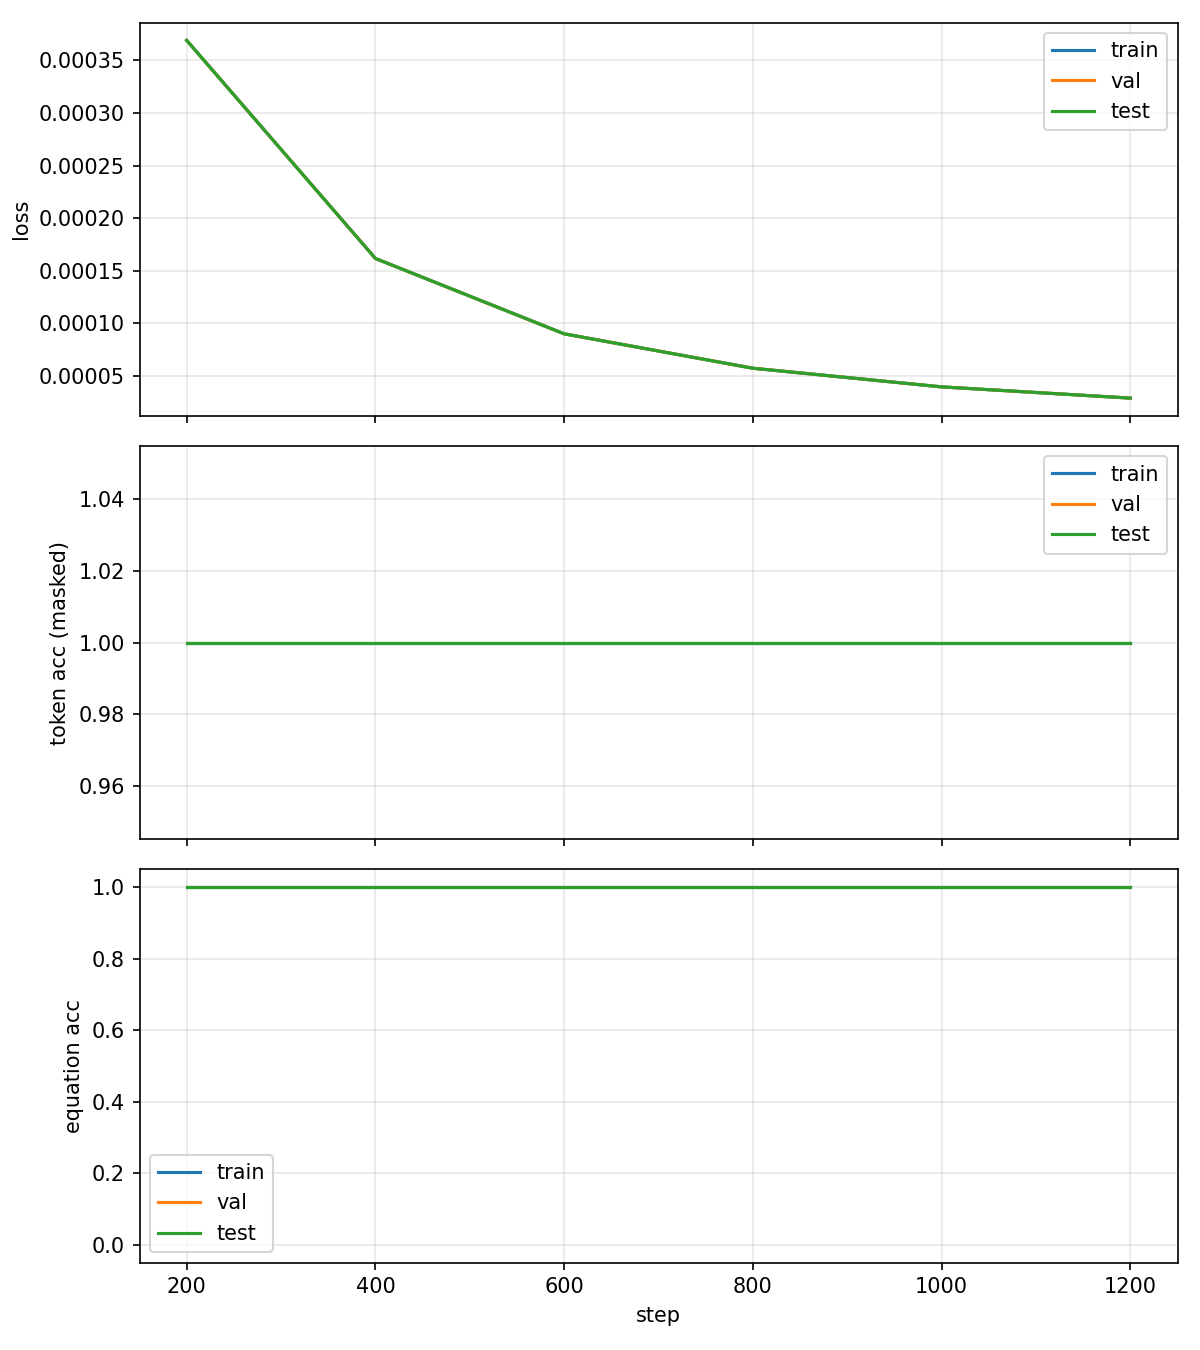
\includegraphics[width=0.85\linewidth]{figures/sanity_suffix.png}
  \caption{Sanity suffix run (loss masked on first three body tokens): metrics (\texttt{runs/sanity\_suffix\_quick}).}
\end{figure}

\subsection*{Modifications and challenges}

\textit{(Brief summary.)} Padding-aware causal attention; causal mask buffer registered for both flash and explicit paths; AdamW returned from \texttt{configure\_optimizers}; YAML configs with seeded RNG; answer-only and suffix masks aligned with shifted cross-entropy.

\section*{Part 1.1: Modular arithmetic data}

\subsection*{Generation command}

\begin{verbatim}
python arith_data.py --seed 0
\end{verbatim}

\noindent
This writes \texttt{data/p\{97,113\}/\{add,sub,div\}/\{train,val,test\}.txt} and \texttt{meta.json} per folder. Equations use the format \texttt{\{a\} \{op\} \{b\} = \{c\}} (decimal digits, spaces). Split: 80\%/10\%/10\% train/val/test after shuffling with seed~0. Division uses all $b\in\{1,\ldots,p-1\}$; addition and subtraction use all $a,b\in\{0,\ldots,p-1\}$.

\subsection*{Dataset sizes}

\begin{center}
\begin{tabular}{@{}rrrrrr@{}}
\toprule
$p$ & op & total & train & val & test \\
\midrule
97 & $+$/$-$ & 9409 & 7527 & 940 & 942 \\
97 & $/$ & 9312 & 7449 & 931 & 932 \\
113 & $+$/$-$ & 12769 & 10215 & 1276 & 1278 \\
113 & $/$ & 12656 & 10124 & 1265 & 1267 \\
\bottomrule
\end{tabular}
\end{center}

\section*{Part 1.2: Warmup (addition/subtraction)}

\subsection*{Specification}

Models use $n_{\mathrm{embd}}=128$, $h=4$ heads, MLP width $4\times 128=512$, AdamW; loss is computed only on answer tokens after `\texttt{=}' (\texttt{loss\_answer\_only:\ true}). Full experiments use \texttt{max\_steps:\ 100000} (\texttt{configs/part1\_2\_*.yaml}). Metrics CSV includes token accuracy on supervised positions and \textbf{equation accuracy} (fraction of examples where every supervised next-token prediction is correct).

\subsection*{Commands executed here}

\textit{Smoke / short runs} (pipeline check; not the full $10^5$ steps required for final submission plots):

\begin{verbatim}
python train.py --config configs/arith_smoke.yaml
python plot_metrics.py --csv runs/part1_2_smoke/metrics.csv --out figures/part1_2_smoke.png
\end{verbatim}

\noindent
\textit{Three short random restarts} for overlay figures only (\texttt{max\_steps=600}, CPU; full runs use \texttt{part1\_2\_p97\_add\_1L\_restart\{1,2,3\}.yaml}):

\begin{verbatim}
python train.py --config configs/part1_2_p97_add_1L_restart1_quick.yaml
python train.py --config configs/part1_2_p97_add_1L_restart2_quick.yaml
python train.py --config configs/part1_2_p97_add_1L_restart3_quick.yaml
python plot_restarts.py \
  --csv runs/part1_2_quick/p97_add_1L_restart1/metrics.csv \
        runs/part1_2_quick/p97_add_1L_restart2/metrics.csv \
        runs/part1_2_quick/p97_add_1L_restart3/metrics.csv \
  --labels seed101 seed202 seed303 \
  --out figures/part1_2_p97_add_1L_restarts_quick.png
\end{verbatim}

\subsection*{Figures (smoke + quick restarts)}

\begin{figure}[h]
  \centering
  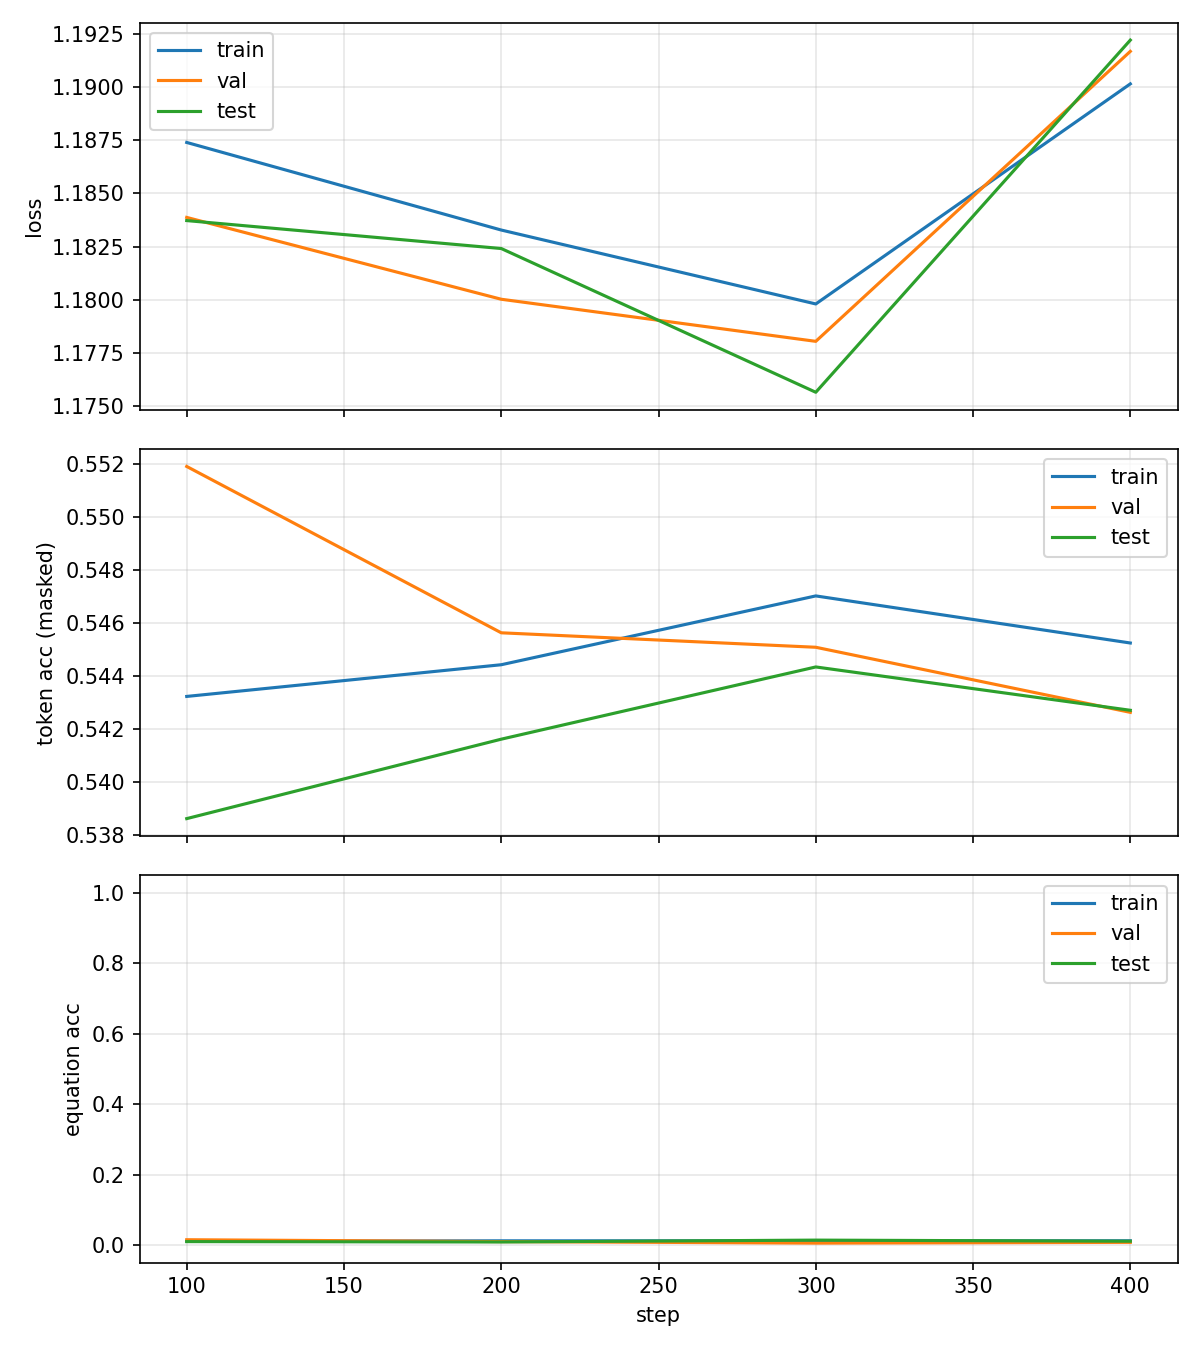
\includegraphics[width=0.85\linewidth]{figures/part1_2_smoke.png}
  \caption{Part 1.2 smoke run ($p{=}97$, addition, 1 layer, 400 steps): loss, token accuracy, equation accuracy (\texttt{runs/part1\_2\_smoke}). Used only to verify logging; train/test have not converged in 400 steps.}
\end{figure}

\begin{figure}[h]
  \centering
  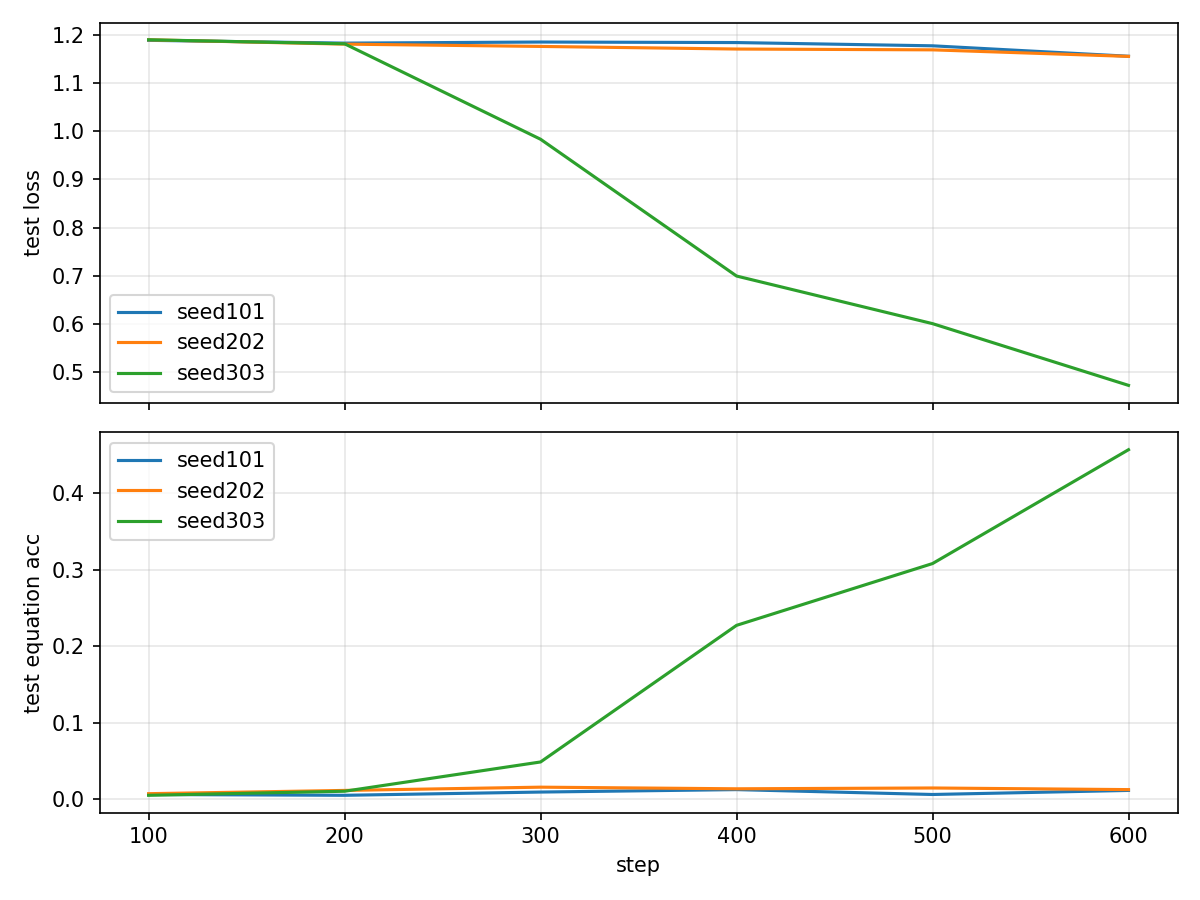
\includegraphics[width=0.85\linewidth]{figures/part1_2_p97_add_1L_restarts_quick.png}
  \caption{Three seeds (101/202/303) for $p{=}97$ addition, 1 layer---\textbf{short} 600-step runs for curve shape only. For the assignment, replace with \texttt{configs/part1\_2\_p97\_add\_1L\_restart\{1,2,3\}.yaml} through $10^5$ steps and submit one checkpoint directory.}
\end{figure}

\subsection*{Full grid (to run for final report)}

\begin{verbatim}
python train.py --config configs/part1_2_p97_add_1L_restart1.yaml
python train.py --config configs/part1_2_p97_add_1L_restart2.yaml
python train.py --config configs/part1_2_p97_add_1L_restart3.yaml
python train.py --config configs/part1_2_p97_add_2L.yaml
python train.py --config configs/part1_2_p97_sub_1L.yaml
python train.py --config configs/part1_2_p97_sub_2L.yaml
python train.py --config configs/part1_2_p113_add_1L.yaml
python train.py --config configs/part1_2_p113_add_2L.yaml
python train.py --config configs/part1_2_p113_sub_1L.yaml
python train.py --config configs/part1_2_p113_sub_2L.yaml
\end{verbatim}

\noindent
After each run: \texttt{python plot\_metrics.py --csv runs/<run>/metrics.csv}. Addition inference demo: load checkpoint then call \texttt{predict\_answer} in \texttt{part\_0\_1\_contract.py} with prompt formatting \texttt{a + b = } (space-separated).

\section*{Part 1.3: Grokking (modular division, $p=97$)}

\subsection*{Setup}

Same architecture as Part~1.2 warmup ($n_{\mathrm{embd}}{=}128$, 4 heads, MLP $512$, answer-only loss). Operation \texttt{op:\ "/"}, modulus \texttt{p:\ 97}. Training uses the same 80/10/10 split (\texttt{split\_seed:\ 0}) as \S1.1. \textbf{Full grokking runs are long} (handout Fig.~1 style); we use \texttt{max\_steps:\ 300000} with periodic eval/save in \texttt{configs/part1\_3\_div\_p97.yaml}.

\subsection*{Commands}

\textit{Full run (submit checkpoint from final \texttt{runs/part1\_3\_div\_p97/}):}

\begin{verbatim}
python train.py --config configs/part1_3_div_p97.yaml
python plot_metrics.py --csv runs/part1_3_div_p97/metrics.csv --out figures/part1_3_div_p97.png
\end{verbatim}

\noindent
\textit{Smoke run executed here} (800 steps, validates division pipeline only---no grokking expected):

\begin{verbatim}
python train.py --config configs/part1_3_div_p97_smoke.yaml
python plot_metrics.py --csv runs/part1_3_div_p97_smoke/metrics.csv \
    --out figures/part1_3_div_p97_smoke.png
\end{verbatim}

\subsection*{Figure (smoke)}

\begin{figure}[h]
  \centering
  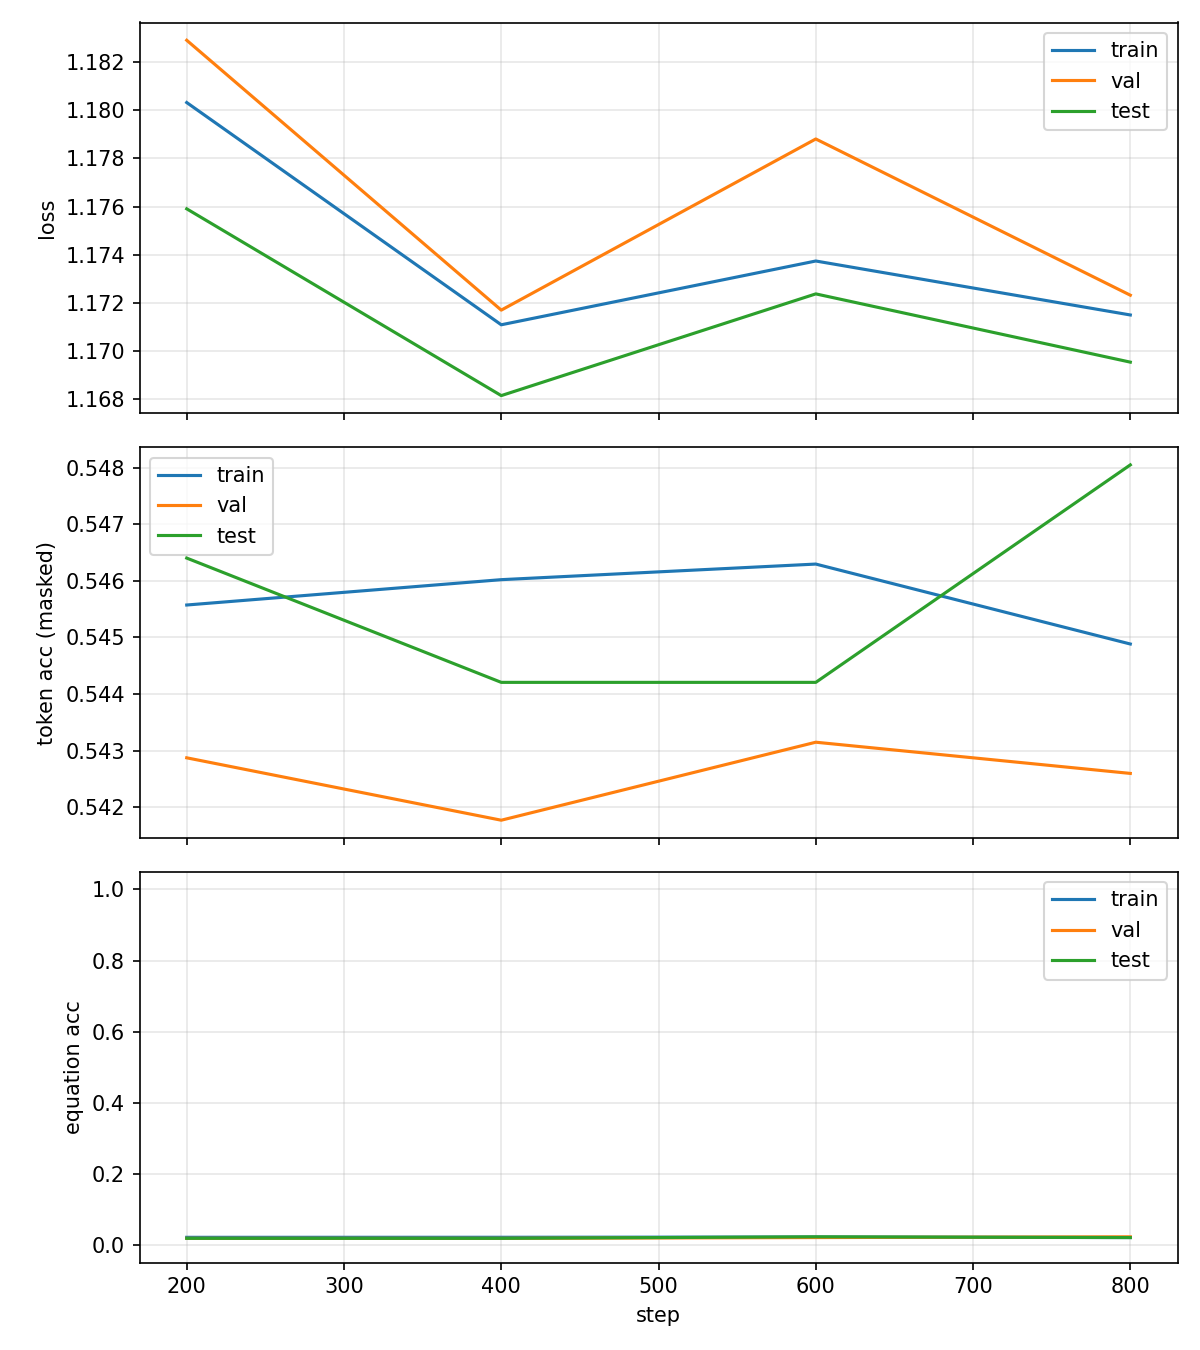
\includegraphics[width=0.85\linewidth]{figures/part1_3_div_p97_smoke.png}
  \caption{Division $p{=}97$, 1 layer---\textbf{short} smoke run (\texttt{runs/part1\_3\_div\_p97\_smoke}). Replace with curves from the full config for the submission plot resembling Fig.~1 (train vs.\ test generalization gap closing after memorization).}
\end{figure}

\subsection*{Inference (division)}

Load the saved run directory (must contain \texttt{tokenizer.json} and \texttt{ckpt\_*.pt}). Example:

\begin{verbatim}
python -c "from part_0_1_contract import load_model_and_tokenizer, predict_answer
m,t = load_model_and_tokenizer('runs/part1_3_div_p97')
print(predict_answer(m, t, 56, 13, '/', 97))"
\end{verbatim}

\noindent
This uses the spaced stem \texttt{a / b = } consistent with \S1.1 formatting.

\section*{Part 1.4: Ablations on division (grokking lag)}

\subsection*{Hypotheses and configs}

We compare the Part~1.3 \textbf{baseline} (\texttt{weight\_decay:\ 1.0}, \texttt{dropout:\ 0}) to two ablations:

\begin{itemize}
  \item \textbf{A --- weaker weight decay:} \texttt{weight\_decay:\ 0.1} (\texttt{configs/part1\_4\_ablation\_wd\_low.yaml}). Motivation: WD controls effective capacity / regularization in grokking (see Power et al.\ and follow-ups); changing it shifts when memorization occurs and how fast test catches up.
  \item \textbf{B --- dropout:} \texttt{dropout:\ 0.2} (\texttt{configs/part1\_4\_ablation\_dropout.yaml}). Motivation: explicit stochastic regularization may alter memorization speed and generalization delay differently than WD alone.
\end{itemize}

\subsection*{Measuring grokking lag}

Script \texttt{analyze\_grokking.py} reads \texttt{metrics.csv} and reports:
\texttt{train\_fit\_step} (first step with train equation accuracy $\geq 0.999$),
\texttt{test\_fit\_step} (first step at or after that with test equation accuracy $\geq 0.999$),
and \texttt{grokking\_lag\_steps} $=$ test fit minus train fit.
Example:

\begin{verbatim}
python analyze_grokking.py --csv runs/part1_3_div_p97/metrics.csv
\end{verbatim}

\noindent
On the short smoke CSVs below, train/test never reach threshold within 800 steps, so lag is \texttt{null}---run full configs for table entries.

\subsection*{Commands (full experiments)}

\begin{verbatim}
python train.py --config configs/part1_3_div_p97.yaml
python train.py --config configs/part1_4_ablation_wd_low.yaml
python train.py --config configs/part1_4_ablation_dropout.yaml
\end{verbatim}

\noindent
Then plot and analyze each run's \texttt{metrics.csv}. Smoke verification (\textbf{executed here}):

\begin{verbatim}
python train.py --config configs/part1_4_ablation_wd_low_smoke.yaml
python train.py --config configs/part1_4_ablation_dropout_smoke.yaml
python plot_restarts.py \
  --csv runs/part1_3_div_p97_smoke/metrics.csv \
        runs/part1_4_ablation_wd_low_smoke/metrics.csv \
        runs/part1_4_ablation_dropout_smoke/metrics.csv \
  --labels baseline wd0.1 dropout0.2 \
  --out figures/part1_4_ablations_div_smoke_compare.png
\end{verbatim}

\subsection*{Figures}

\begin{figure}[h]
  \centering
  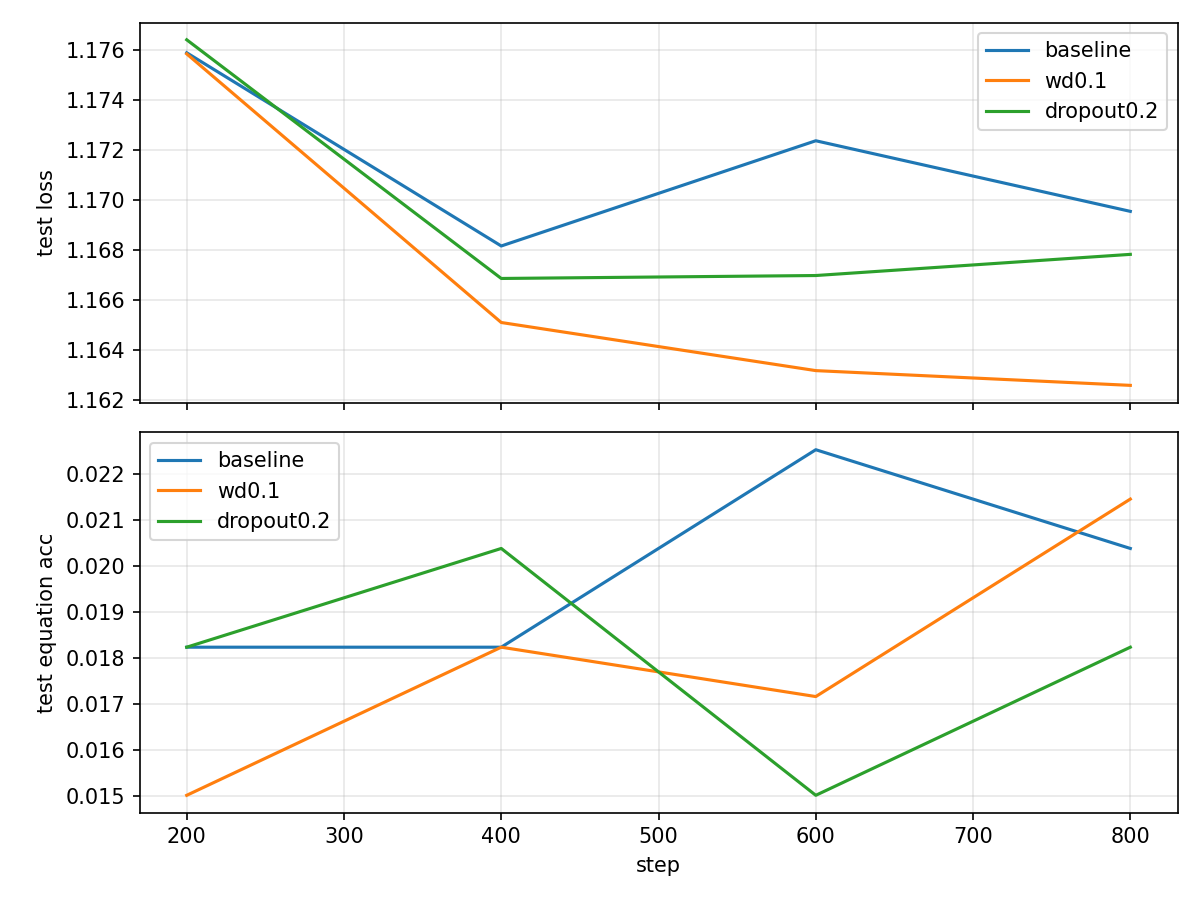
\includegraphics[width=0.85\linewidth]{figures/part1_4_ablations_div_smoke_compare.png}
  \caption{Overlay of \textbf{smoke} division runs: baseline vs.\ WD ablation vs.\ dropout (test loss and test equation accuracy). For the report, regenerate after full $3{\times}10^5$ step runs and fill in grokking lag from \texttt{analyze\_grokking.py}.}
\end{figure}

\begin{figure}[h]
  \centering
  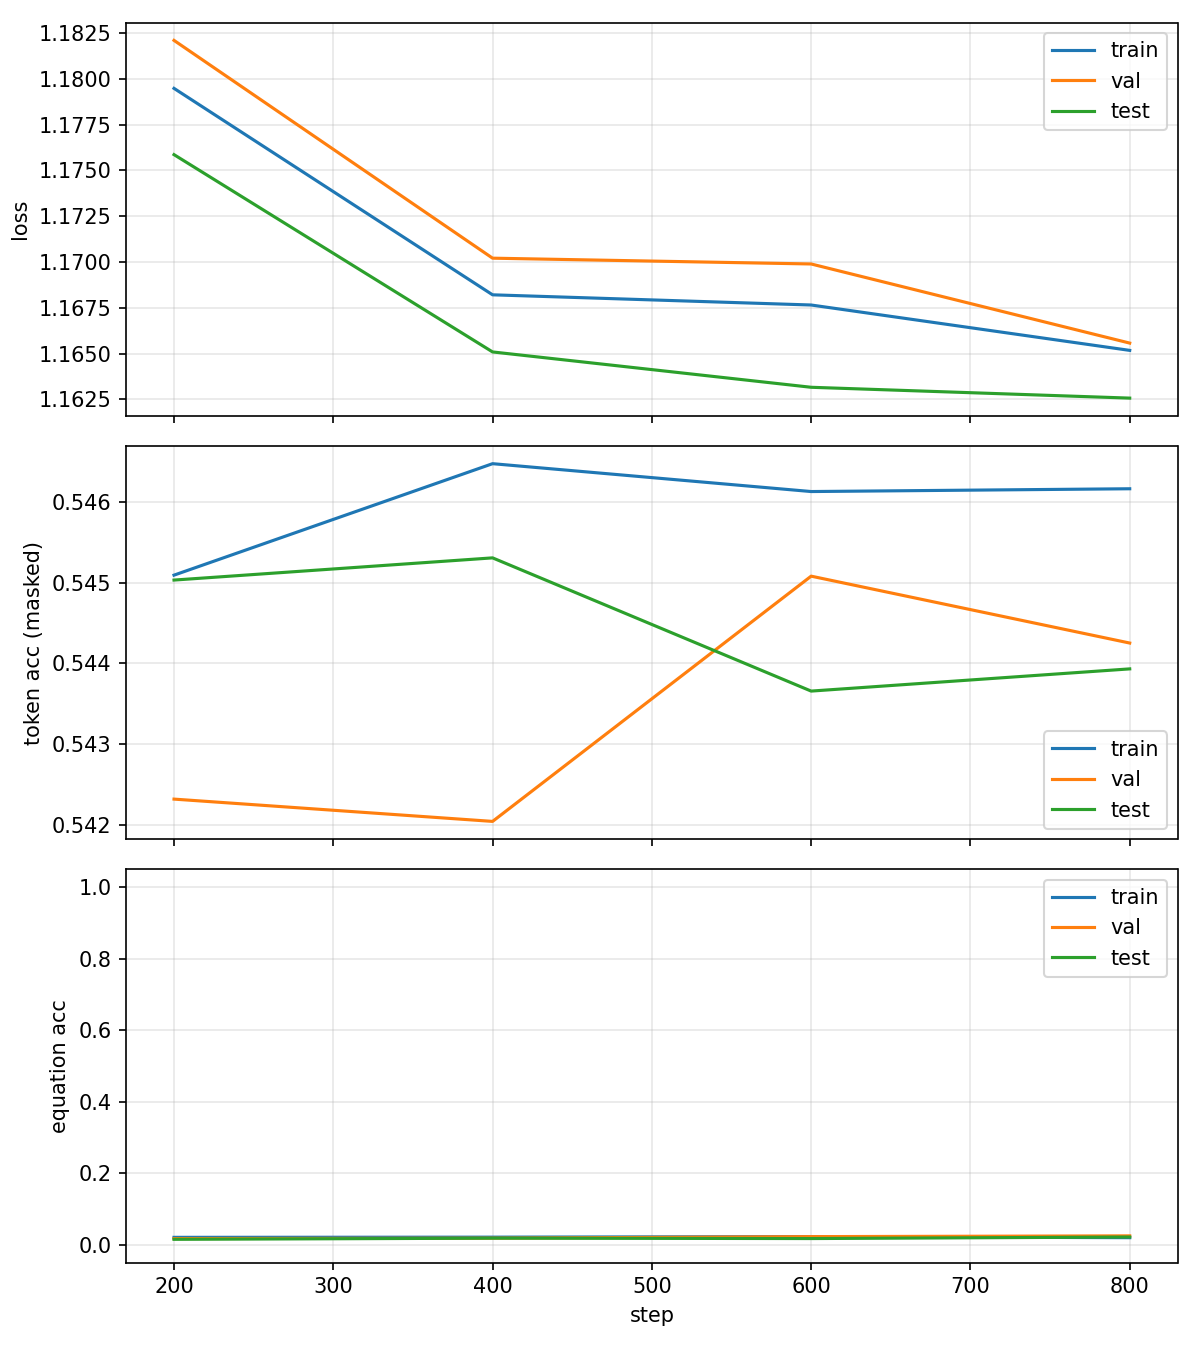
\includegraphics[width=0.42\linewidth]{figures/part1_4_wd_low_smoke.png}
  \hfill
  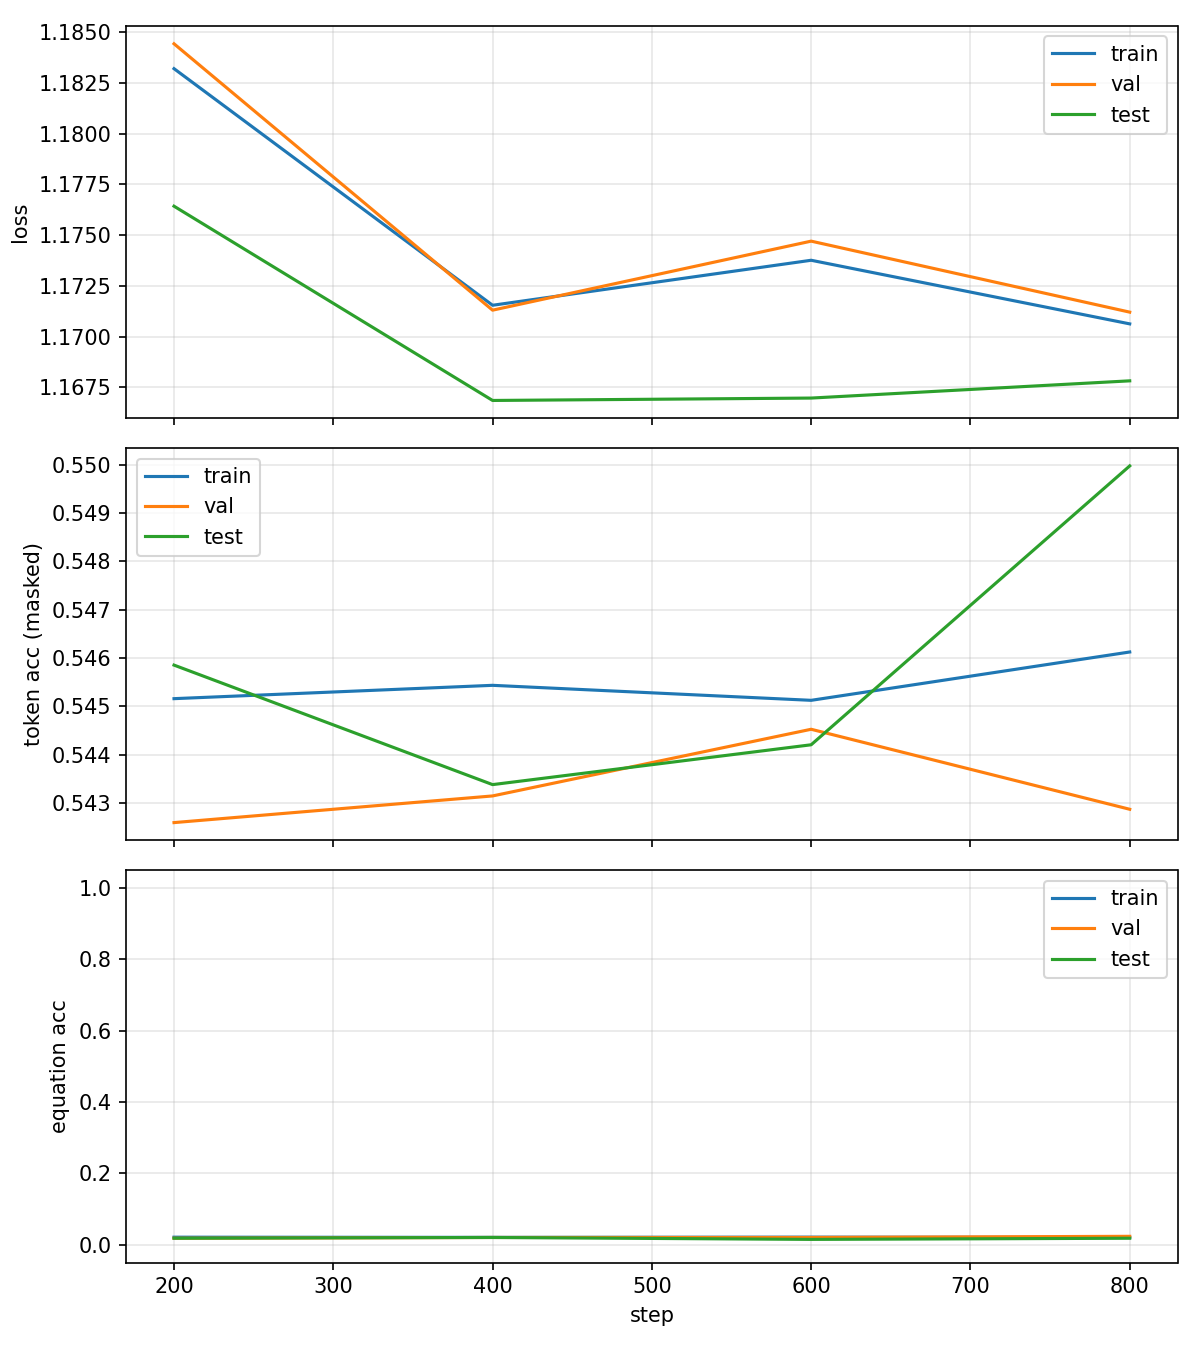
\includegraphics[width=0.42\linewidth]{figures/part1_4_dropout_smoke.png}
  \caption{Individual smoke plots: WD ablation (left), dropout ablation (right).}
\end{figure}

\subsection*{Placeholder results table (fill after full runs)}

\begin{center}
\begin{tabular}{@{}lccc@{}}
\toprule
Run & Train-fit step & Test-fit step & Grokking lag \\
\midrule
Baseline (\texttt{part1\_3\_div\_p97}) & --- & --- & --- \\
WD $0.1$ (\texttt{part1\_4\_ablation\_wd\_low}) & --- & --- & --- \\
Dropout $0.2$ (\texttt{part1\_4\_ablation\_dropout}) & --- & --- & --- \\
\bottomrule
\end{tabular}
\end{center}

\end{document}
